\section{Gaußoptik}
\subsection{ABCD-Gesetz in der geometrischen Optik}
In der paraxialen Optik wird die Veränderung von Lichtstrahlen mithilfe von Matrizen dargestellt. Diese nennt 
man aufgrund ihrer vier Einträge auch ABCD-Matrix.\\
Diese wurde eingeführt, da man komplizierter Sachverhalte, z.B. eine Kugelwelle, in der Optik oft nicht ausreichend genau mit einen
Strahlenvektor darstellen kann. \\
Jeder Strahl lässt sich durch den Abstand $r$ zur optischen Achse und dem Winkel $\alpha$, den der Strahl 
mit der opt. Achse einschließt, beschreiben.
Man kann diesen Strahl mithilfe dieser beiden Komponenten darstellen:

$\vec{v}= \left(\begin{array}{c} r \\ \alpha \end{array}\right)$

\begin{figure}[h]
    \centering
    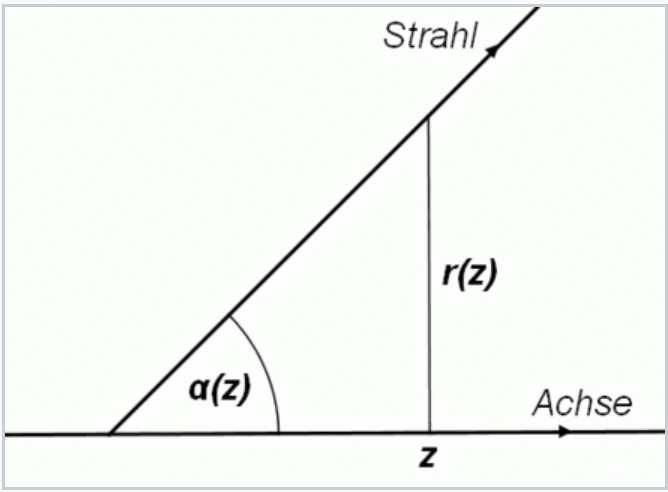
\includegraphics[scale=0.4]{Bilder/FzV/gaus.png}
    \caption{Graphische Darstellung des Vektors $\vec{v}$. }
\end{figure}
Unter Verwendung der Kleinwinkelnäherung gilt für den Krümmungsradius der Kugelwelle vor dem optischen System:
\begin{equation}
    R_1 = \frac{x_1}{\alpha_1}
\end{equation}
Und analog gilt für den Krümmungsradius der Kugelwelle nach dem optischen System:
\begin{equation}
    R_2 = \frac{x_2}{\alpha_2}
\end{equation}
Die Beziehung zwischen den zwei Vektoren $\vec{v}_1$ und $\vec{v}_2$ kann man aus der Transformationsmatrix T erhalten. \citep[vgl.][]{optik} \\
\begin{align}
    T = \left(\begin{array}{rr} 
    A & B  \\ 
    C & D \\ 
    \end{array}\right)\\
    x_2 = Ax_1 + B\alpha_1\\
    \alpha_2 = Cx_1 + D\alpha_1
\end{align}
Daraus folgt für den Krümmungsradius $R_2$:
\begin{equation}
    R_2  = \frac{x_2}{\alpha_2} = \frac{AR_1 + B}{C R_1 + D}
\end{equation}
\newpage
\subsection{Gaußstrahlen}
Die Gaußstrahlen sind ein Konzept zur Beschreibung der Lichtausbreitung, hierbei werden  
sowohl die Methoden der Strahlenoptik als auch der Wellenoptik verwendet.
Die gerade angesprochene geometrische Optik lässt sich auch auf die Gaußstrahlen übertragen. 
Gaußstrahlen sind Strahlen, die einer Gauß-Verteilung der Amplitude folgen.\\ 
Hier gibt es statt den Strahlenvektor einen Strahlenparameter $q$:
\begin{equation}
    q = \frac{A q_0 + C}{C q_o + D}
\end{equation}
Der Strahlenparameter berechnet sich hierbei wie folgt:
\begin{equation}
    \frac{1}{q} = \frac{1}{R} - \frac{i \lambda }{\pi \omega^2}
\end{equation}
$R$ steht für den Krümmungsradius des Gauß-Strahls, $\lambda$ für dessen Wellenlänge und $\omega$ für den Radius des Gauß-Strahls. \citep[vgl.][]{optik}

\subsection{Der Strahlausbreitungsfaktor M$^2$}
Ein realer Laserstrahl weist nur selten ein ideales Gaußprofil auf, sondern es kommt zur Abweichung des Laserprofils durch Überlagerungen
verschiedener Moden, um eine Möglichkeit zu nennen. 
Man führt aus diesem Grund den Strahlungsausbreitungsfaktor $M^2$ ein, dieser gibt an wie weit der reale Strahl 
vom theoretischen Gaußstrahl abweicht.
